\documentclass[aspectratio=169]{beamer}
\mode<presentation>

\usepackage{calc}
\usepackage{relsize}
\usepackage{graphicx}
\usepackage[overlay,absolute]{textpos}

\graphicspath{{../images}}

\usepackage{fontspec}
\setsansfont{Helvetica Neue Light}[BoldFont={Helvetica Neue Bold}]
\setmonofont{Iosevka Term}
\newfontface\helvreg{Helvetica Neue}

\title{My favorite programming languages}
\subtitle{and three others}
\author{Douglas Creager\\\textsmaller[1]{\href{https://dcreager.net/}{@dcreager}}\vspace{-0.5em}}
\institute{
\includegraphics[width=2.5em]{github-mark.pdf}\vspace{2em}}
\date{Craft Conf\\\textsmaller[1]{June 2, 2022 – Budapest}}

\newlength{\titlewidth}
\newcommand{\flattitle}[3]{
    \settowidth{\titlewidth}{\textbf{\LARGE #3}}
    \begin{textblock*}{\titlewidth}(#1,#2)
        \textbf{\LARGE #3}
    \end{textblock*}
}
\newcommand{\shadowedtitle}[3]{
    \settowidth{\titlewidth}{\textbf{\LARGE #3}}
    \addtolength{\titlewidth}{0.5mm}
    \begin{textblock*}{\titlewidth}(#1+0.4mm,#2+0.4mm)
        \textbf{\LARGE #3}
    \end{textblock*}
    \begin{textblock*}{\titlewidth}(#1,#2)
        \textbf{\textcolor{white}{\LARGE #3}}
    \end{textblock*}
}

\setbeamercolor{title}{fg=black}
\setbeamerfont{title}{series=\bfseries,size=\larger[1]}
\setbeamercolor{frametitle}{fg=black}
\setbeamerfont{frametitle}{series=\bfseries}

\setbeamerfont{institute}{size=\normalsize}

\setbeamertemplate{navigation symbols}{}

% Picture credits

\makeatletter
\def\picturecredits{}
\newcommand{\picturecredit}[4]{\picturecreditraw{#1}{#2}{#3}{\url{#4}}}
\newcommand{\picturecreditraw}[4]{
    \protected@xappto\picturecredits{
        \textsmaller[3]{Slide \theframenumber} &
        \textsmaller[2]{#1, “#2”} \vspace*{-0.4em} \newline
        \textsmaller[3]{#3, #4} \\
    }
}
\makeatother

\begin{document}

\begin{frame}
    \titlepage
\end{frame}

\begin{frame}
    %\begin{textblock*}{160mm}(0mm,-15mm)
    %    \only<1>{
    %    \picturecreditraw
    %      {Pieter Bruegel the Elder}
    %      {The Tower of Babel (Rotterdam)}
    %      {Public domain}
    %      {\href{https://commons.wikimedia.org/wiki/File:Pieter_Bruegel_the_Elder_-_The_Tower_of_Babel_(Rotterdam)_-_Google_Art_Project_-_edited.jpg}{Wikimedia Commons}}
    %    }
    %    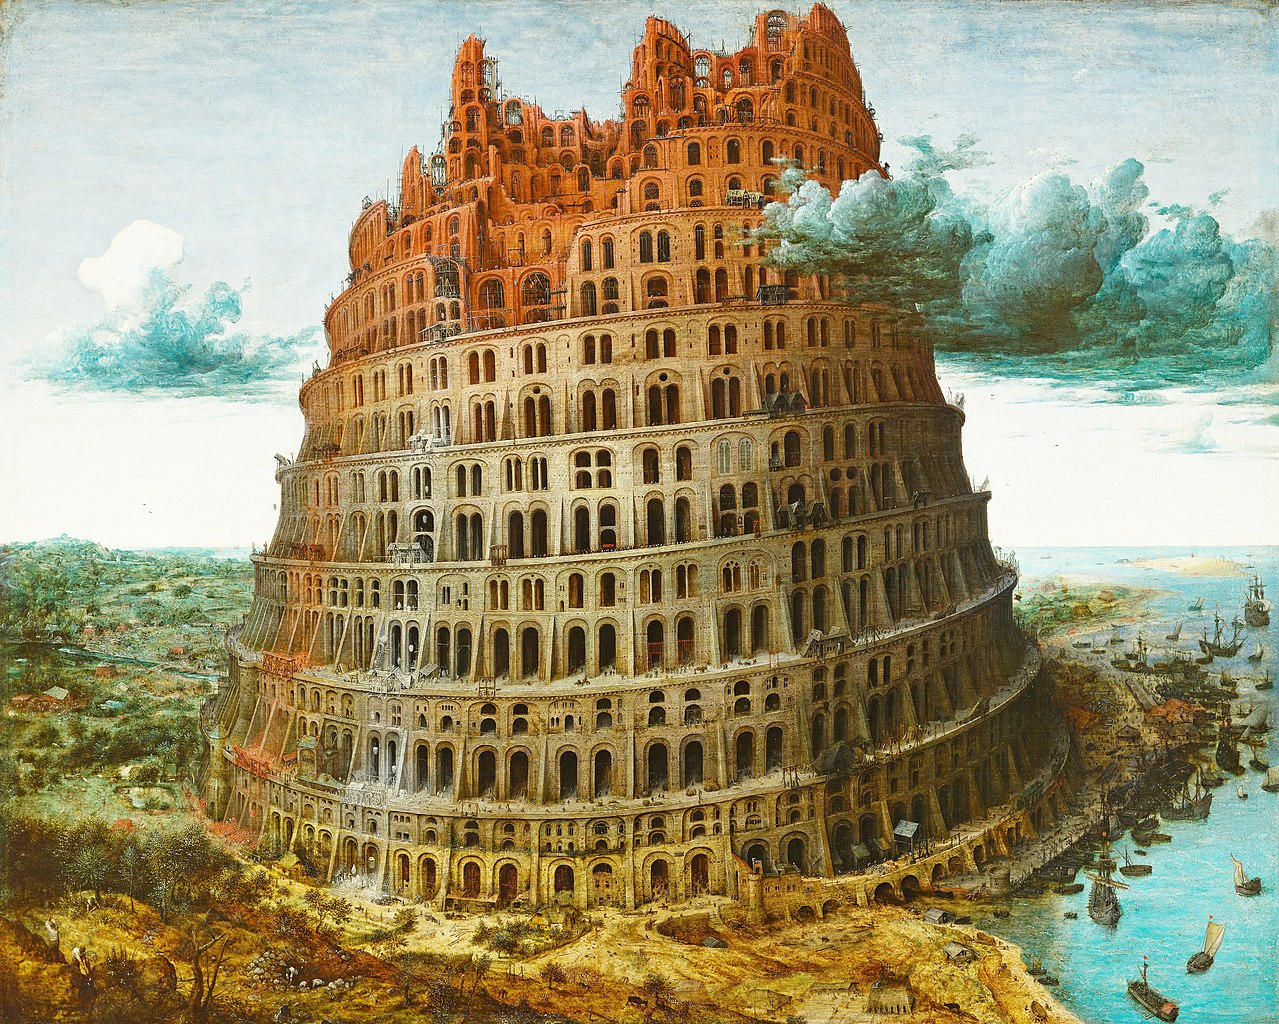
\includegraphics[width=160mm]{tower-of-babel-bruegel.jpg}
    %\end{textblock*}
    \begin{textblock*}{160mm}(5mm,5mm)
        \only<1>{
        \picturecredit
          {Meister der Weltenchronik}
          {Weltchronik in Versen, Szene: Der Turmbau zu Babel}
          {Public domain}
          {https://commons.wikimedia.org/wiki/File:Meister_der_Weltenchronik_001.jpg}
        }
        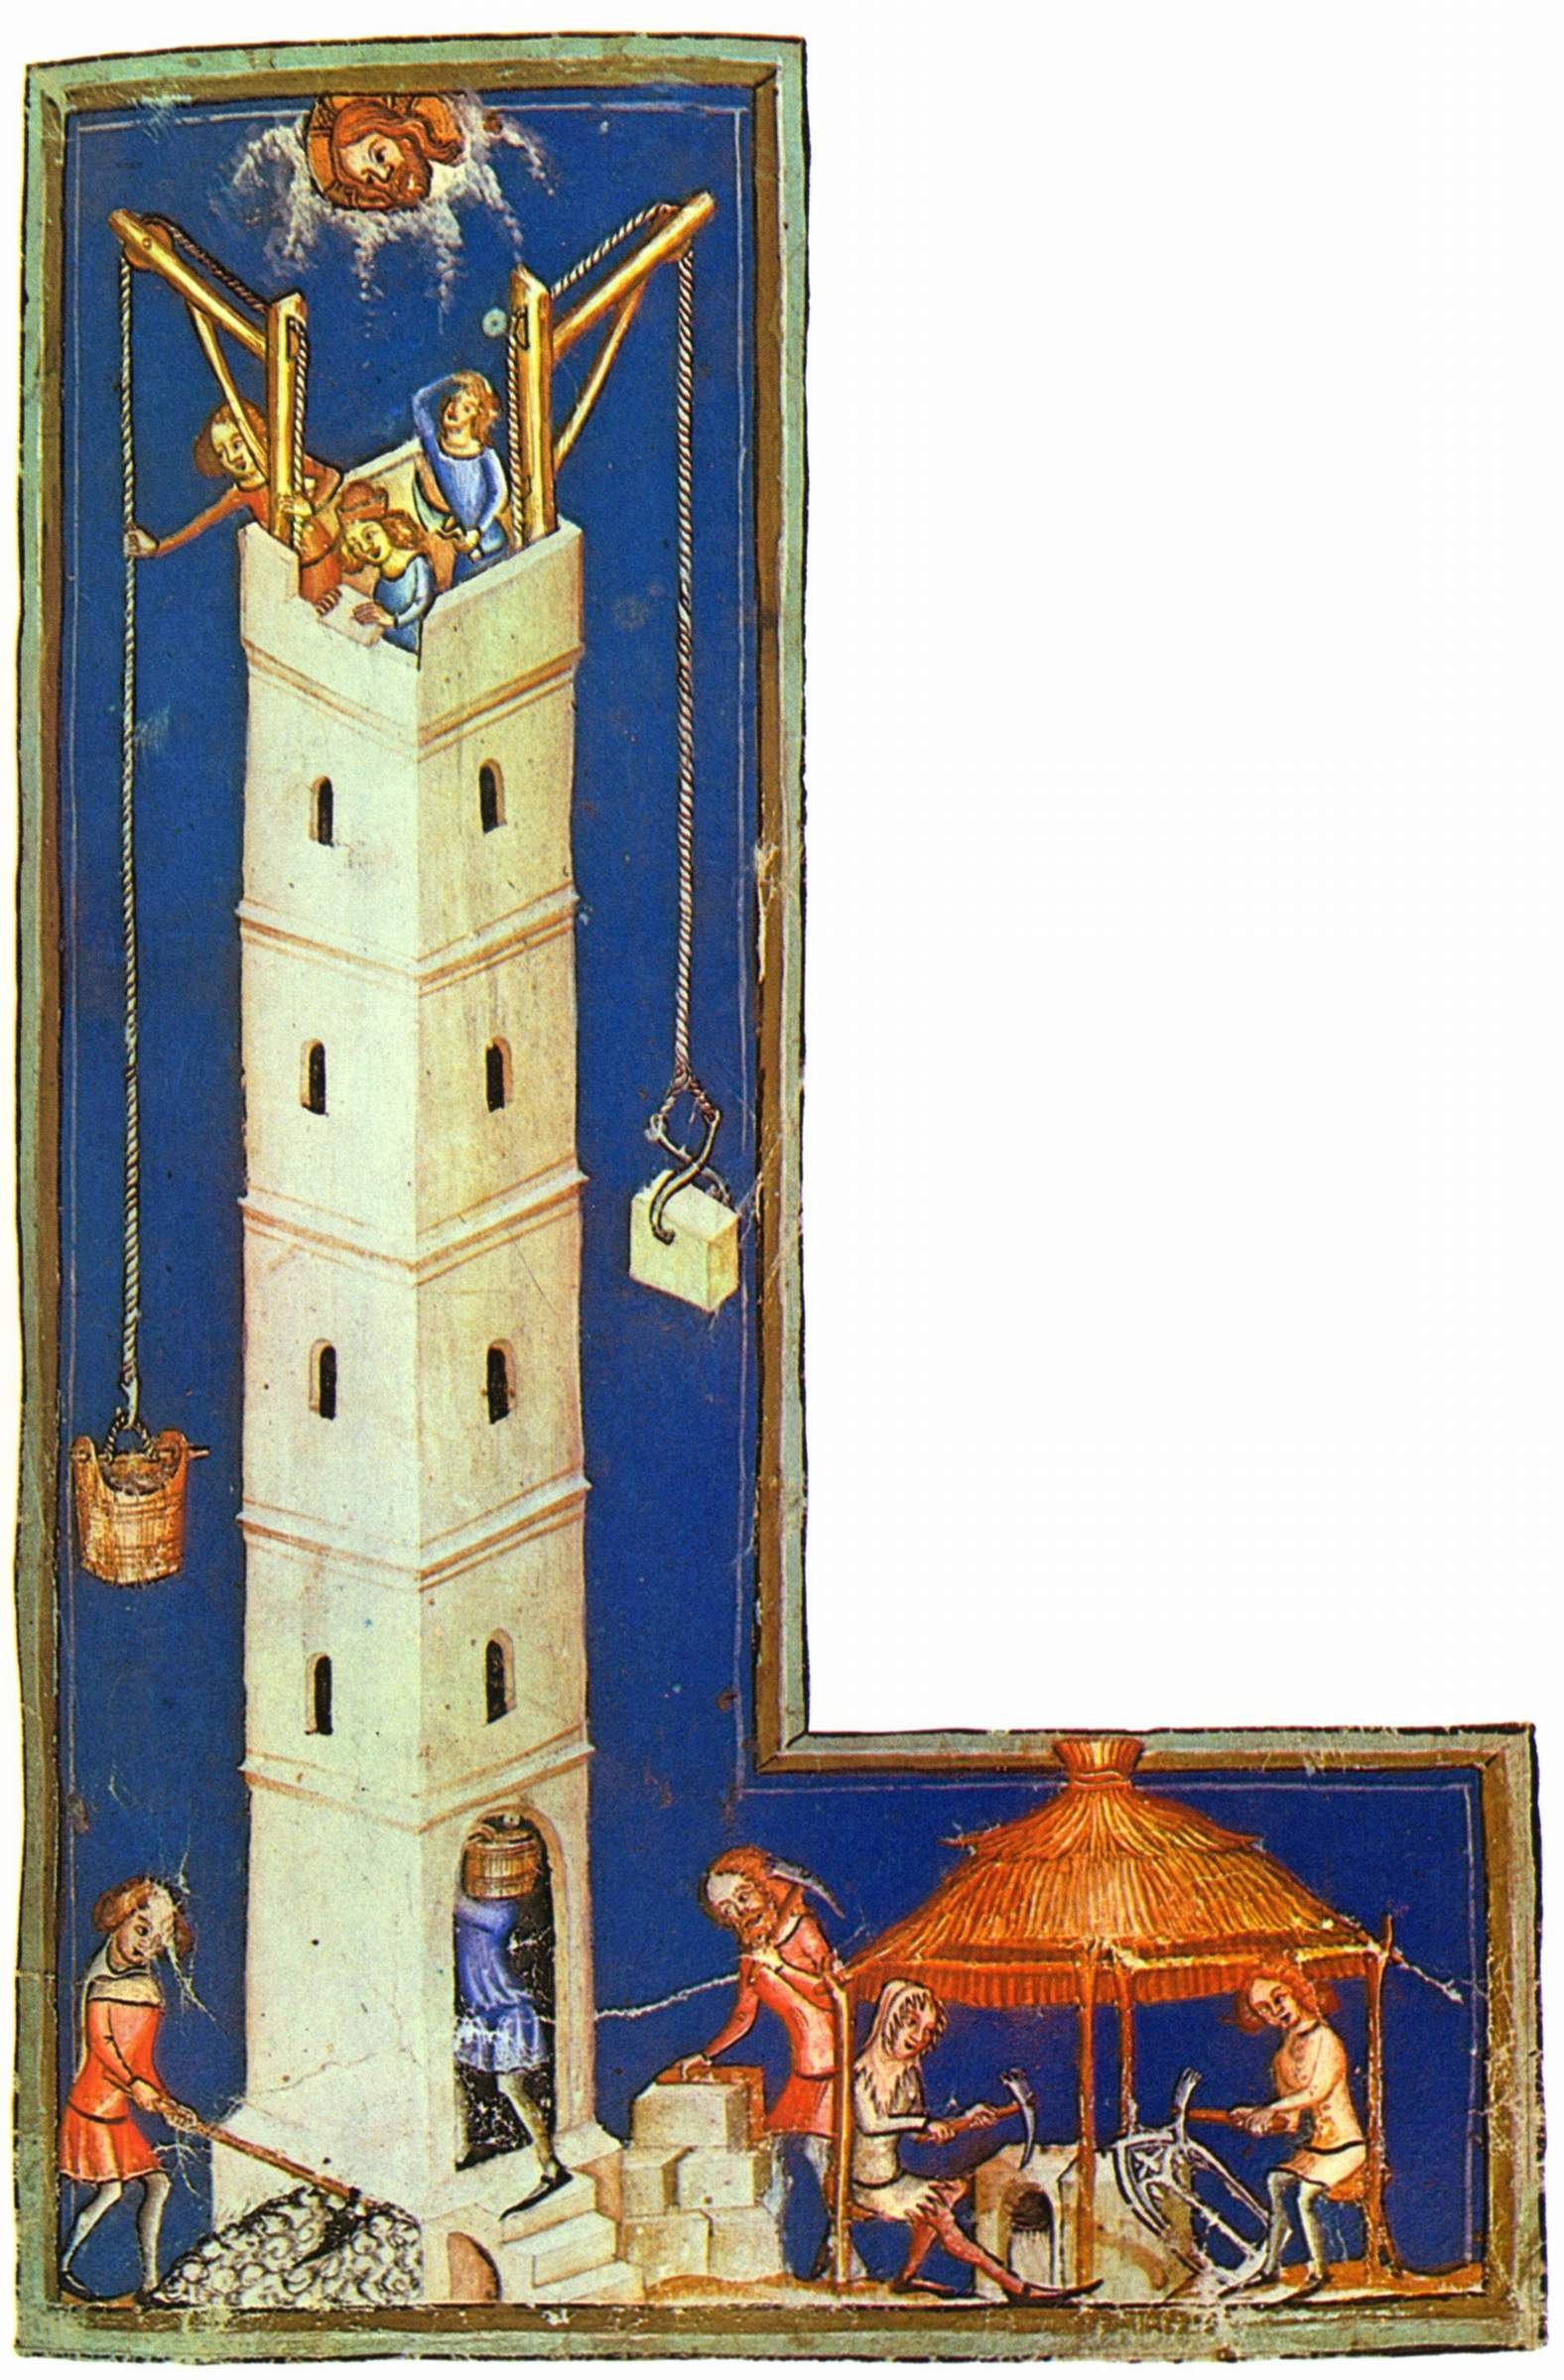
\includegraphics[height=80mm]{tower-of-babel-weltenchronik.jpg}
    \end{textblock*}

    \begin{textblock*}{15mm}( 86mm,-1mm)
        \only<3>{
\includegraphics[width=8mm]{languages/python.png}}
    \end{textblock*}
    \begin{textblock*}{15mm}( 98mm,-1mm)
        \only<3>{
\includegraphics[width=8mm]{languages/csharp.png}}
    \end{textblock*}
    \begin{textblock*}{15mm}(110mm,-1mm)
        \only<3>{
\includegraphics[width=8mm]{languages/perl.png}}
    \end{textblock*}
    \begin{textblock*}{15mm}(122mm,-1mm)
        \only<3>{
\includegraphics[width=8mm]{languages/ruby.png}}
    \end{textblock*}

    \begin{textblock*}{15mm}( 86mm,11mm)
        \only<3>{
\includegraphics[width=8mm]{languages/haskell.png}}
    \end{textblock*}
    \begin{textblock*}{15mm}( 98mm,11mm)
        \only<3>{
\includegraphics[width=8mm]{languages/nim.png}}
    \end{textblock*}
    \begin{textblock*}{15mm}(110mm,11mm)
        \only<3>{
\includegraphics[width=8mm]{languages/javascript.png}}
    \end{textblock*}
    \begin{textblock*}{15mm}(122mm,11mm)
        \only<3>{
\includegraphics[width=8mm]{languages/c.png}}
    \end{textblock*}

    \begin{textblock*}{15mm}( 86mm,23mm)
        \only<3>{
\includegraphics[width=8mm]{languages/bash.png}}
    \end{textblock*}
    \begin{textblock*}{15mm}( 98mm,23mm)
        \only<3>{
\includegraphics[width=8mm]{languages/elixir.png}}
    \end{textblock*}
    \begin{textblock*}{15mm}(110mm,23mm)
        \only<3>{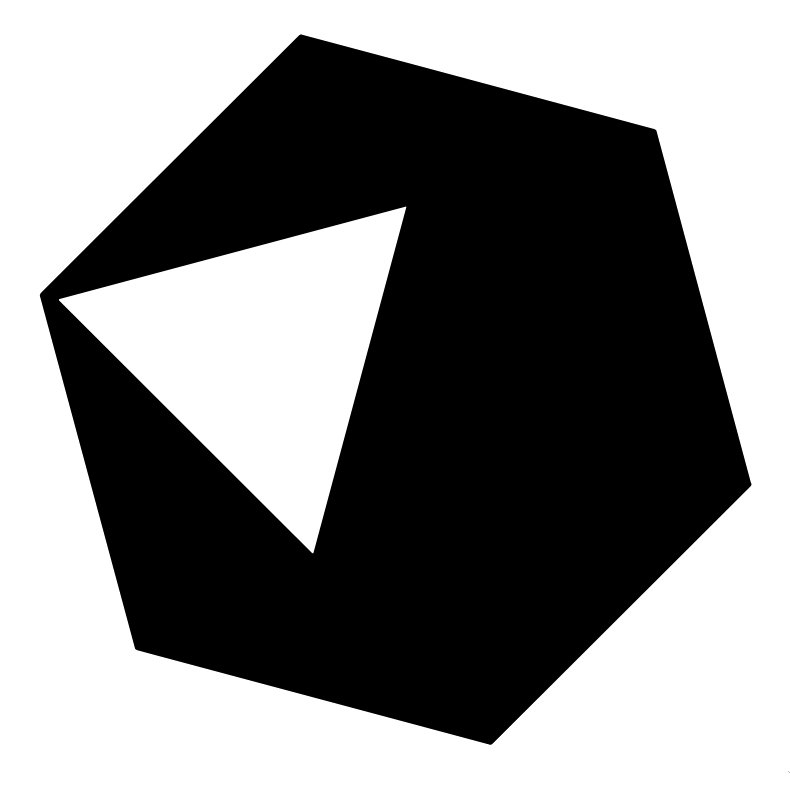
\includegraphics[width=8mm]{languages/crystal.png}}
    \end{textblock*}
    \begin{textblock*}{15mm}(122mm,23mm)
        \only<3>{
\includegraphics[width=8mm]{languages/racket.png}}
    \end{textblock*}

    \begin{textblock*}{15mm}( 86mm,35mm)
        \only<3>{
\includegraphics[width=8mm]{languages/dart.png}}
    \end{textblock*}
    \begin{textblock*}{15mm}( 98mm,35mm)
        \only<2-3>{
\includegraphics[width=8mm]{languages/fortran.png}}
    \end{textblock*}
    \begin{textblock*}{15mm}(110mm,35mm)
        \only<3>{
\includegraphics[width=8mm]{languages/ocaml.png}}
    \end{textblock*}
    \begin{textblock*}{15mm}(122mm,35mm)
        \only<3>{
\includegraphics[width=8mm]{languages/kotlin.png}}
    \end{textblock*}

    \begin{textblock*}{15mm}( 86mm,47mm)
        \only<3>{
\includegraphics[width=8mm]{languages/cpp.png}}
    \end{textblock*}
    \begin{textblock*}{15mm}( 98mm,47mm)
        \only<3>{
\includegraphics[width=8mm]{languages/scala.png}}
    \end{textblock*}
    \begin{textblock*}{15mm}(110mm,47mm)
        \only<2-3>{
\includegraphics[width=8mm]{languages/cobol.png}}
    \end{textblock*}
    \begin{textblock*}{15mm}(122mm,47mm)
        \only<3>{
\includegraphics[width=8mm]{languages/swanson.png}}
    \end{textblock*}

    \begin{textblock*}{15mm}( 86mm,59mm)
        \only<3>{
\includegraphics[width=8mm]{languages/java.png}}
    \end{textblock*}
    \begin{textblock*}{15mm}( 98mm,59mm)
        \only<3>{
\includegraphics[width=8mm]{languages/erlang.png}}
    \end{textblock*}
    \begin{textblock*}{15mm}(110mm,59mm)
        \only<3>{
\includegraphics[width=8mm]{languages/zig.png}}
    \end{textblock*}
    \begin{textblock*}{15mm}(122mm,59mm)
        \only<3>{
\includegraphics[width=8mm]{languages/php.png}}
    \end{textblock*}

    \begin{textblock*}{15mm}( 86mm,71mm)
        \only<3>{
\includegraphics[width=8mm]{languages/typescript.png}}
    \end{textblock*}
    \begin{textblock*}{15mm}( 98mm,71mm)
        \only<3>{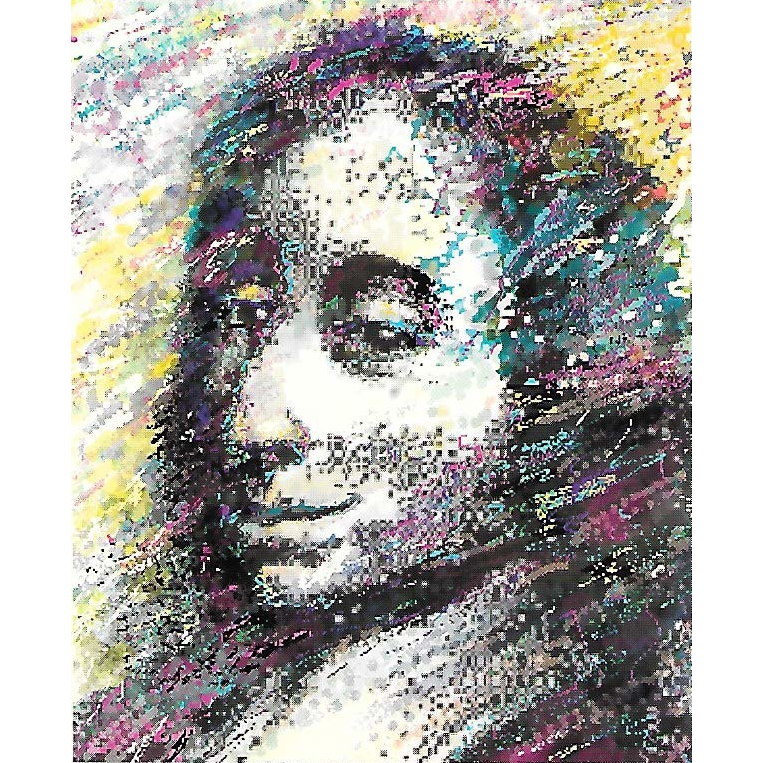
\includegraphics[width=8mm]{languages/turbo-pascal.png}}
    \end{textblock*}
    \begin{textblock*}{15mm}(110mm,71mm)
        \only<3>{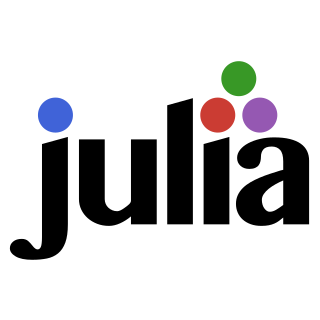
\includegraphics[width=8mm]{languages/julia.png}}
    \end{textblock*}
    \begin{textblock*}{15mm}(122mm,71mm)
        \only<3>{
\includegraphics[width=8mm]{languages/r.png}}
    \end{textblock*}

    \begin{textblock*}{15mm}( 86mm,83mm)
        \only<3>{
\includegraphics[width=8mm]{languages/swift.png}}
    \end{textblock*}
    \begin{textblock*}{15mm}( 98mm,83mm)
        \only<3>{
\includegraphics[width=8mm]{languages/clojure.png}}
    \end{textblock*}
    \begin{textblock*}{15mm}(110mm,83mm)
        \only<3>{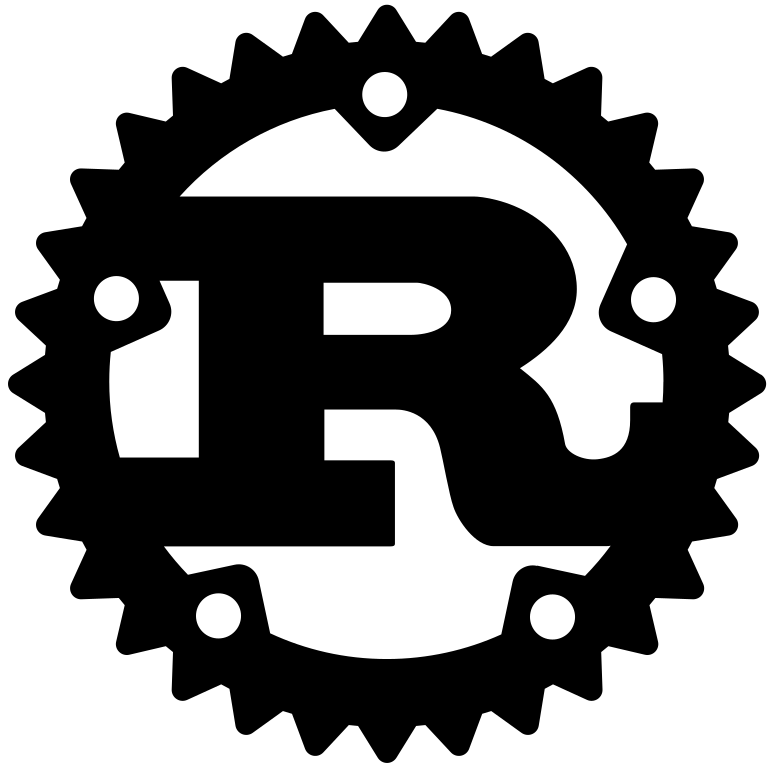
\includegraphics[width=8mm]{languages/rust.png}}
    \end{textblock*}
    \begin{textblock*}{15mm}(122mm,83mm)
        \only<3>{
\includegraphics[width=8mm]{languages/go.png}}
    \end{textblock*}
\end{frame}

\begin{frame}
    \begin{textblock*}{160mm}(0mm,-15mm)
        \picturecredit{Matjaž Mirt}{Tern/čigra}{CC-BY-2.0}{https://flic.kr/p/2kXydKp}
        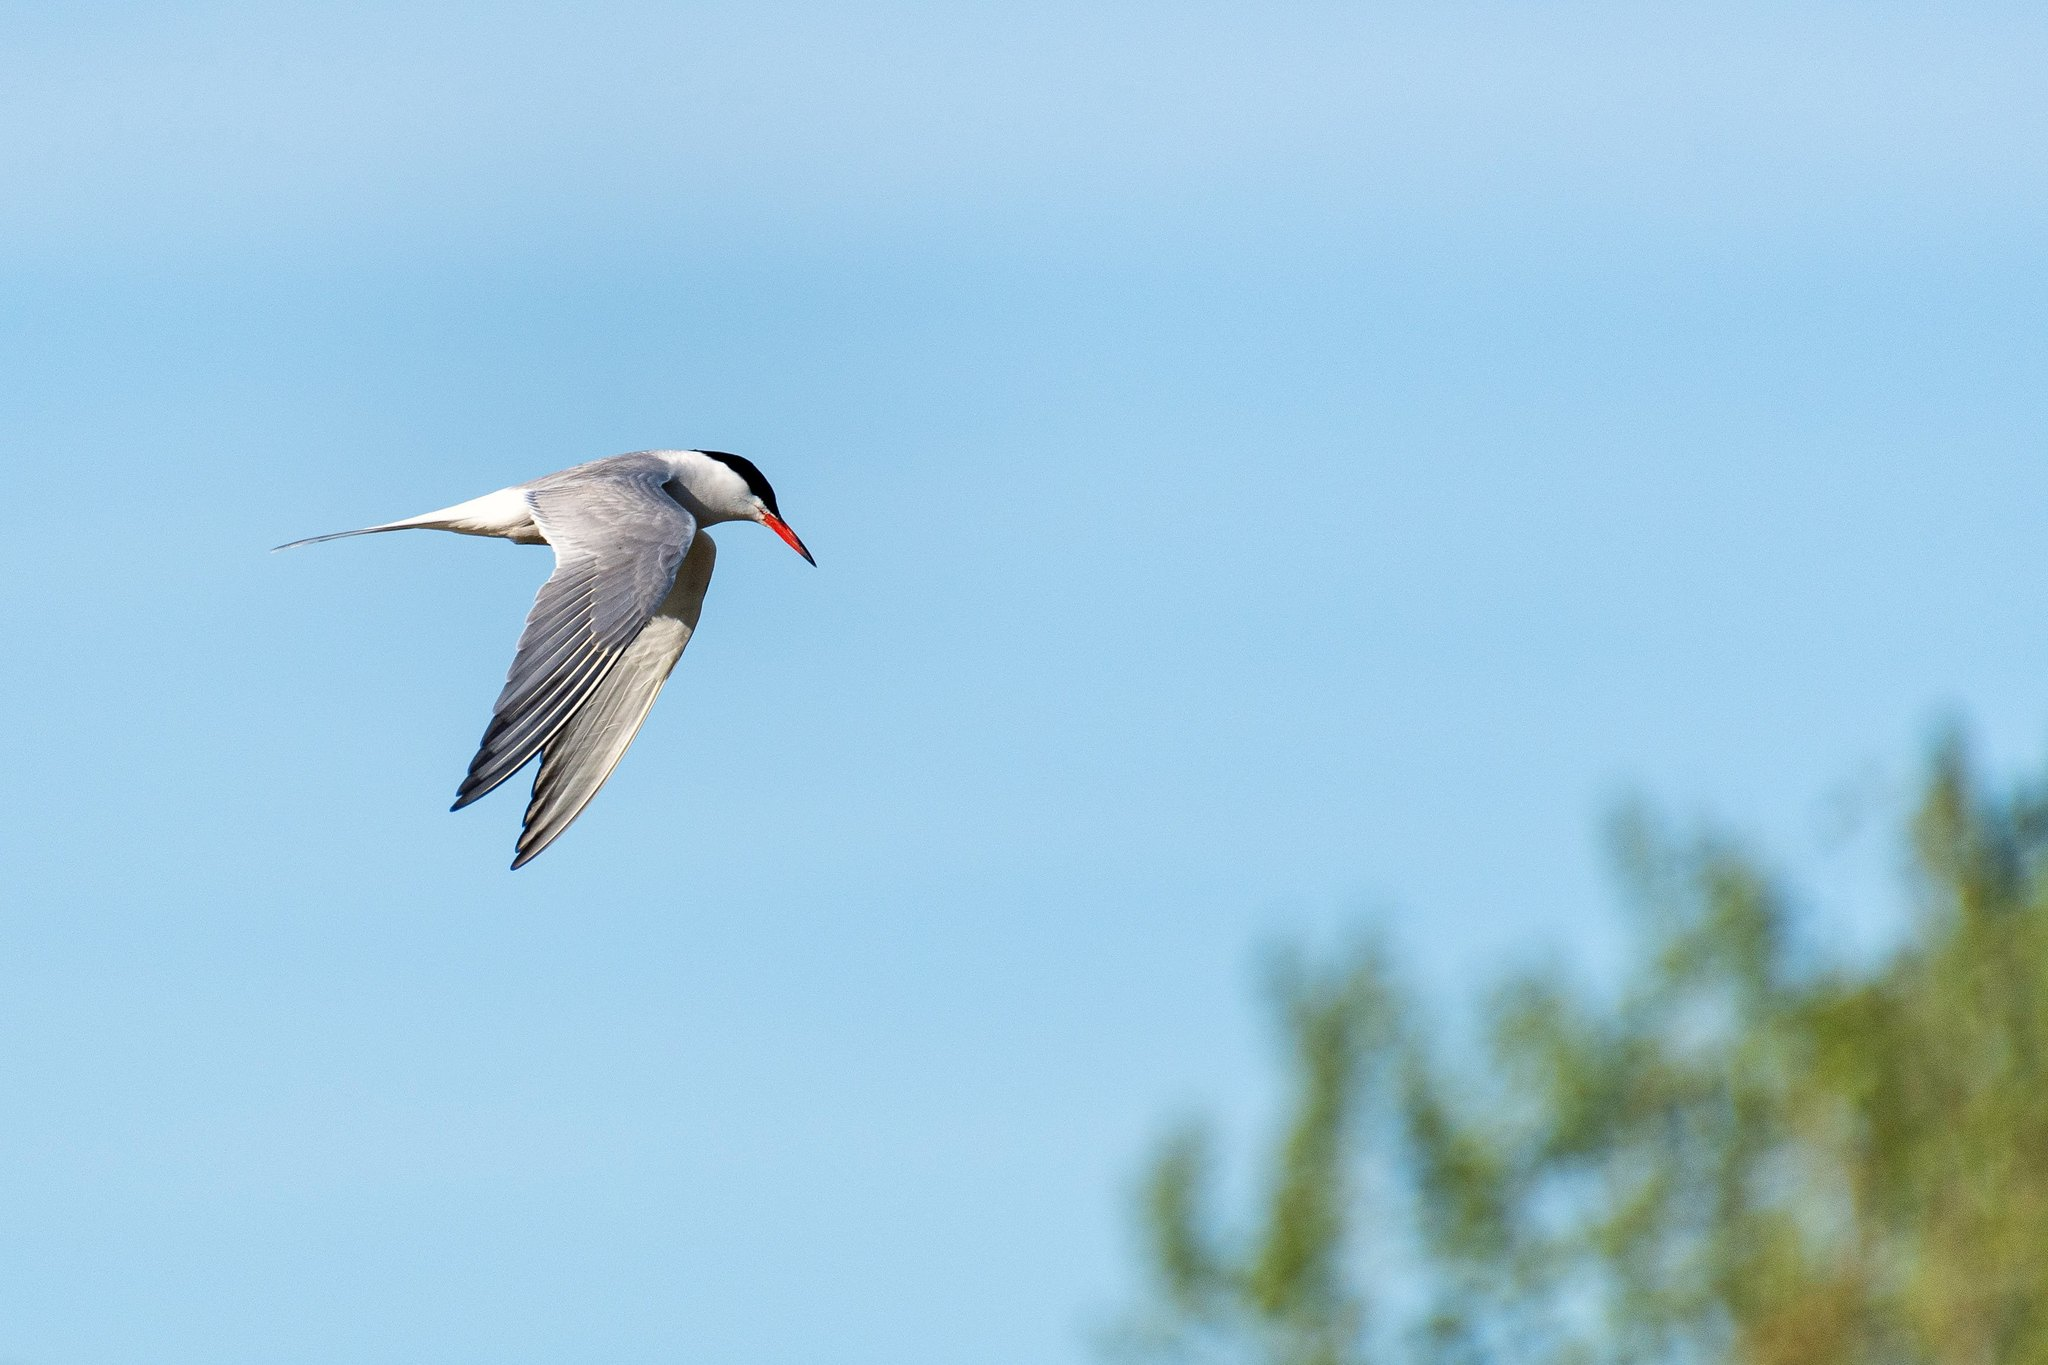
\includegraphics[width=160mm]{one-tern.jpg}
    \end{textblock*}
    \shadowedtitle{150mm - \titlewidth}{10mm}{Isolated languages}
\end{frame}

\begin{frame}
    \begin{textblock*}{160mm}(0mm,0mm)
        \picturecredit{Mark Gunn}{This just tern'ed into a swarm!}{CC-BY-2.0}{https://flic.kr/p/P11JH1}
        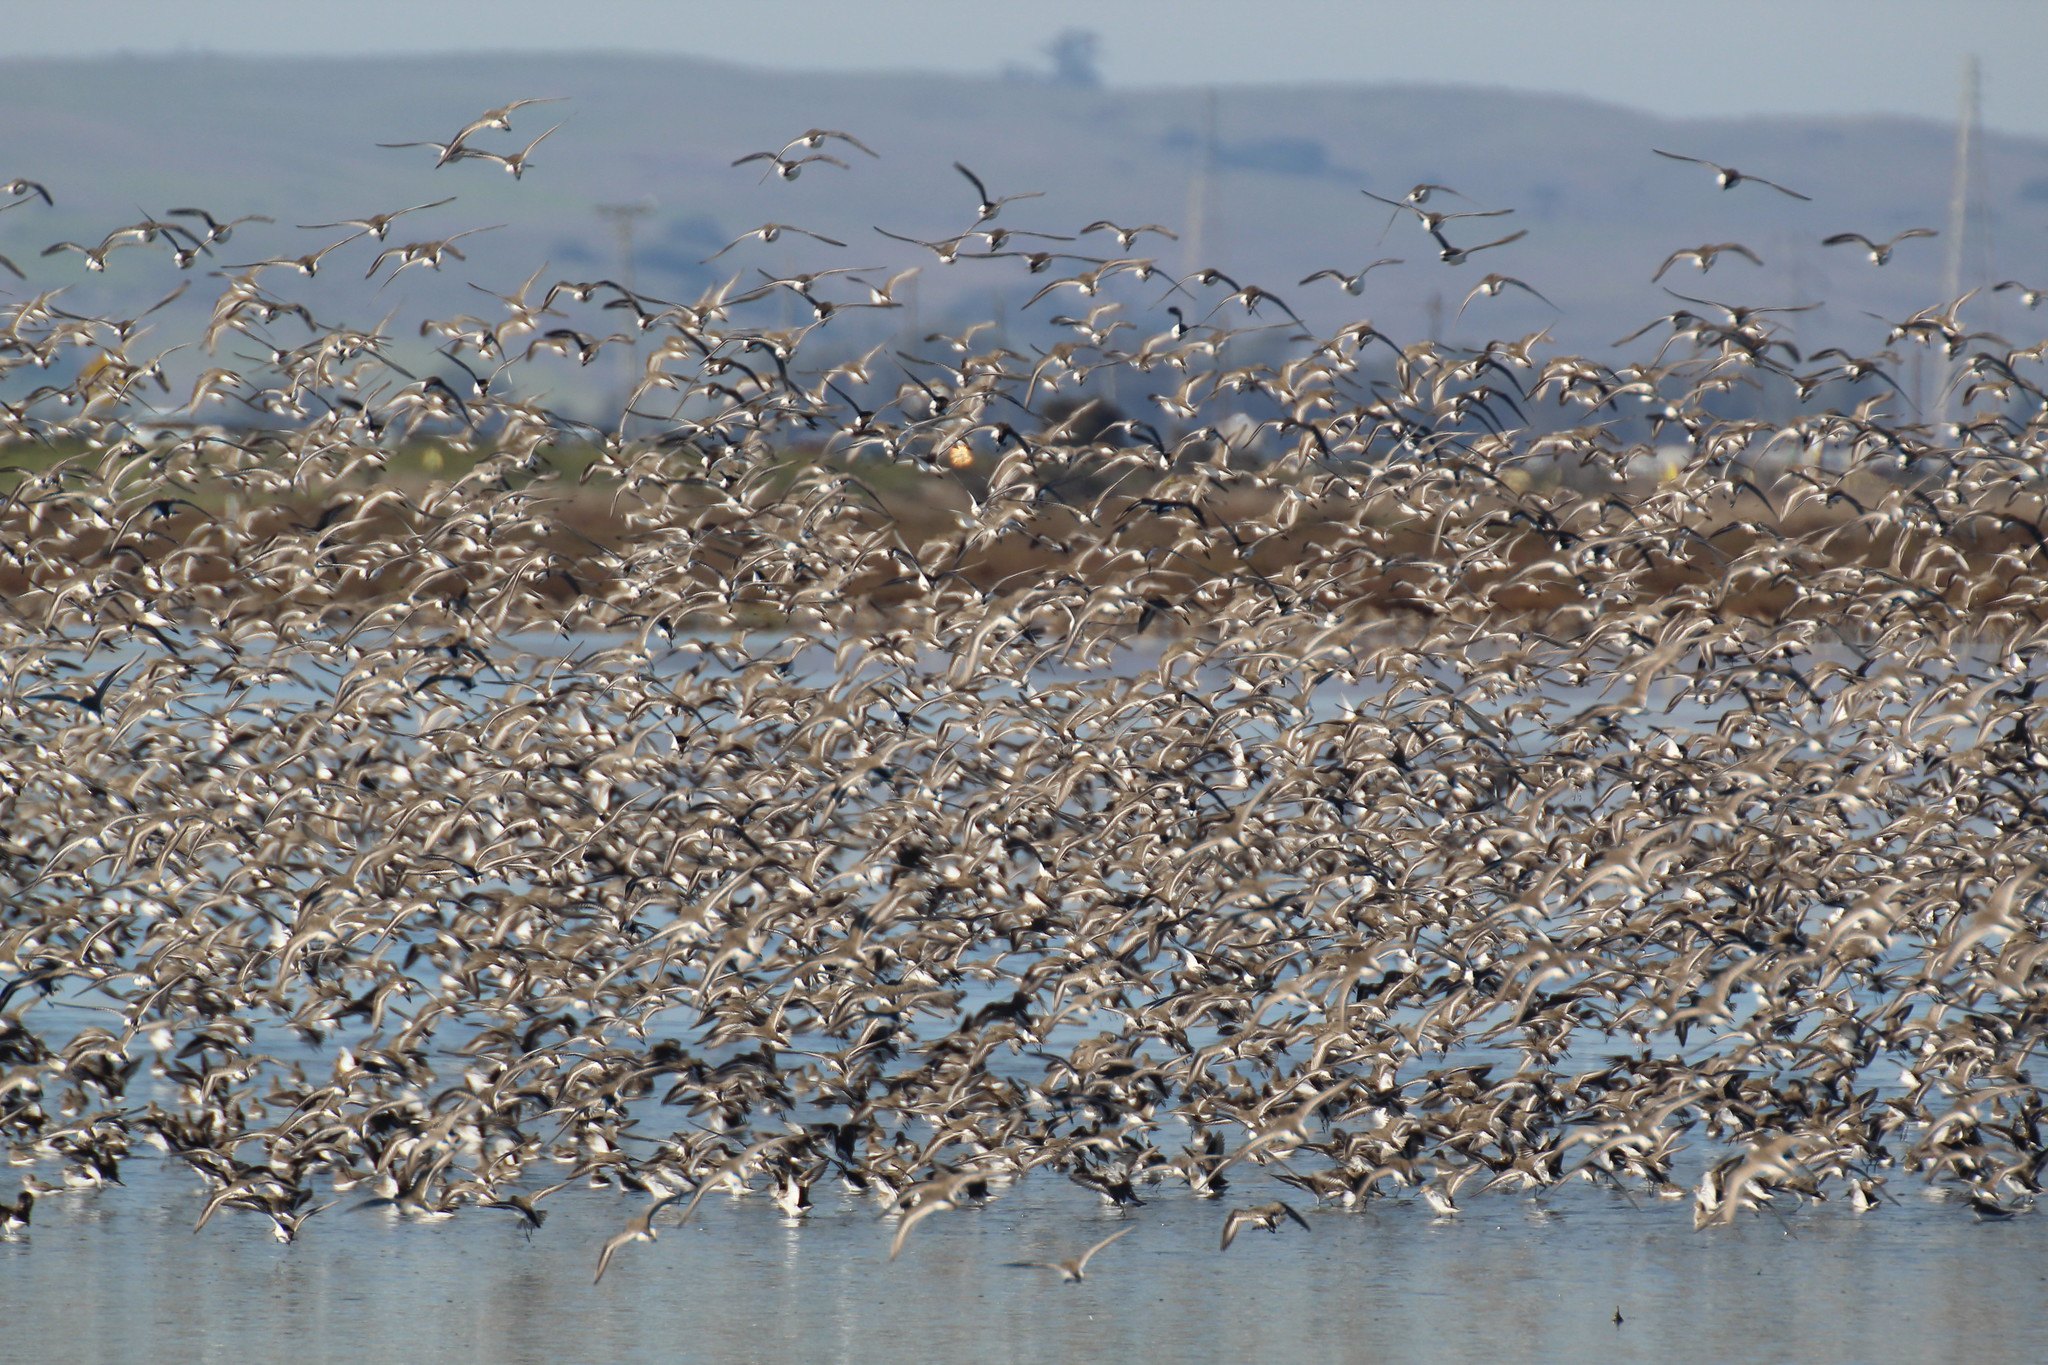
\includegraphics[width=160mm]{terns.jpg}
    \end{textblock*}
    \shadowedtitle{150mm - \titlewidth}{10mm}{Many languages}
\end{frame}


\begin{frame}[t]
    \frametitle{Picture credits}
    \begin{tabular}{lp{0.75\textwidth}}
    \picturecredits
    \end{tabular}
\end{frame}

\end{document}
